\documentclass[10pt,a4paper]{article}
\usepackage[utf8]{inputenc}
\usepackage{amsmath}
\usepackage{amsfonts}
\usepackage{amssymb}
\usepackage{makeidx}
\usepackage{graphicx}
\usepackage{fullpage}
\usepackage{tikz}
\usepackage{pdflscape}

\usepackage{enumitem}% http://ctan.org/pkg/enumitem
\usepackage{graphicx}
\graphicspath{ {images/} }
\usetikzlibrary{arrows,shapes,positioning,shadows,trees,mindmap}
\date{\vspace{-5ex}}
%\date{}  % Toggle commenting to test

\tikzset{
	basic/.style  = {draw, text width=2cm, drop shadow, font=\sffamily, rectangle},
	root/.style   = {basic, rounded corners=2pt, thin, align=center,
		fill=green!30},
	level 2/.style = {basic, rounded corners=6pt, thin,align=center, fill=green!60,
		text width=8em},
	level 3/.style = {basic, thin, align=left, fill=pink!60, text width=6.5em}
}

\title{Stochastik Zusammenfassung}
\begin{document}
	\maketitle
	\section{Beschreibende Statistik}
	\subsection{Merkmalstypen}
	\begin{itemize}
		\item 	qualitativ: Familienstand, Schulnoten. Nominal, ordinal, dichotom
		\item	quantitativ/metrisch: verhältnisskaliert (skalen haben Nullpkt.), diskret, stetig, absolutskaliert (verhältnisskaliert + Nur eine Skala, bspw. Anzahl)
		\item klassiertes Merkmal: Intervall
	\end{itemize}
	\subsection{Median/Quantile}
	
	Median ergibt sich aus der Rangwertreihe, er ist das 0.5 Quantil (p)
	\subsection{Streuungsmaaße}
	\begin{itemize}
		\item Empirische Varianz: Jeder Wert minus den Durchschnitt im Quadrat nehmen und durch die Anzahl der Werte teilen. Sagt etwas über die Verteilung der Werte
		\item Standardabweichung = Wurzel aus Varianz
		\item Kovarianz: $$s_{xy} = \frac{1}{n}  \sum_{i=1}^{n} x_i y_i \cdot \bar x \bar y$$
		\item Spannweite max minus min
		\item mittlere absolute Abweichung: Median $\tilde{x}$ statt Durchschnitt $\bar{x}$
		\item Variazionskoeffizient: Standardabweichung/Durchschnitt	
		\item Quartilskoeffizient: $Q_{koeff}$= 2* Quartilsabstand/(Quartilswertunteres Quartil+Quartilswert oberes Quartil)
		\item Standarisierung/lineare Transformation: $z_i=\frac{x_i-\bar{x}}{s_x	}$
	\end{itemize}
	\subsection{Empirische Verteilungsfunktion}
	Nützlich für Stetige Merkmale, da diese sonst nicht darstellbar. Anzahl der Werte bis zu einem Bestimmten Wert um zu klassifizieren, zusammenzählen der Werte inkl. Häufigkeit.\\
	\includegraphics[scale=0.2]{verteilungsfkt.png}
	\includegraphics[scale=0.2]{verteilungsfkt2.png}

	\subsection{Malen nach Zahlen}
	\begin{itemize}
		\item Säulendiagramm/Stabdiagramm für relative Häuf.
		\item Kreisdiagramm (Pie Chart)
		\item Box-Plot\\ \includegraphics[scale=0.3]{boxplot.png}
		\item Histogramm Die Fläche des Rechtecks über dem Intervall K j ist proportional zur relativen Häufigkeit
		\item Scatterplot/Streudiagramm
	\end{itemize}
	 \subsection{Bravais-Pearson-Korrelationskoeffizient}
	 Kovarianz/(Standardabweichung1*Standardabweichung2). auch berechenbar für linear transformierte Daten. Am besten Arbeitstabelle anfertigen.\\
	 \begin{equation}
	 r_{xy} =
	 \begin{cases}
	 -1/+1 & \text {linearer Zusammenhang, gegensinnig/gleichsinnig} \\
	 0 & \text{unkorreliert/kein linearer Zusammenhang} \\
	 \text{negativ/positiv} & \text{negativ/positiv korreliert}  \\
	 <0.5/\geq 0.5 & \text{schwach/stark korreliert}
	 \end{cases}
	 \end{equation}
	 \subsection{Regressionsanalyse}
	 Liefert funktionalen Zusammenhang 
	 \begin{itemize}
	   \item Y wird als Regressand bzw. als abhängige Variable bezeichnet.
	   \item f heißt Regressionsfunktion.
	   \item Die Werte: y i = f ( x i ) , i = 1 ,..., n, heißen Regressionswerte .
	   \item $\epsilon$ =  Fehlerterm, da die tatsächlichen Werte von $y_i$ in der Regel nicht getroffen werden
		\item Bestimmtheitsmaß sagt aus wie naha die Regressionsgerade an den tatsächlichen Werten liegt (1 = bester Wert)	
	 \end{itemize}
	
	\section{Wahrscheinlichkeitsrechnung}
	
	\subsection{Begriffe}
	\begin{enumerate}
		\item Momentbegriff: Ein Moment schließt Erwartungswert, etc. ein und ist der Oberbegriff dafür. Ein Moment gilt für einen bestimmten Wert einer Zufallsvariable. Beim Moment wird integriert.
		\item $\sigma_0$ = bekannte Varianz
		\item Erwartungstreue von Schätzern: Erwartungstreu wenn erwartungswert gleich dem des zu schätzenden Parameters, Abweichung=Verzerrung/Bias
		\item Verteilungsfunktion $F^x(x)=P(X\leq x)$ ich lese also immer ab die Wahrsch. ob kleiner gleich, sonst muss ich diese per 1-x negieren.
	\end{enumerate}
	\subsection{Varianz Rechenregeln}
	$Var(-2Y)=4\space Var(Y)$
	\subsection{bedingte Wahrscheinlichkeit Rechenregeln}
	\begin{itemize}
		\item S13 Formelsammlung. $P(A|B)=\frac{P(A\cap B)}{P(B)}$
		\item $P(A\cap B)=P(B\cap A)$
		\item Seite 11 die ganzen Regeln
		\item Außerdem zu beachten: ${P(B\cup C | A)} = P(B|A)+P(C|A) - P(B\cap C | A)$
	\end{itemize}
	\subsection{Modelieren mit Zufallsvariable und Angabe von Verteilung}
	Angabe der möglichen Ausprägungen in einem Wahrscheinlichkeitsraum $(\Omega,\mathfrak{A},P)$ und Angabe der jeweiligen Wahrscheinlichkeiten für die Belegungen $P(X=A)=$ Wahrscheinlicheit. Meistens kann dann eine Verteilungsfkt gefunden werden, bspw. Binomialverteilung.
	\subsection{Urnenmodelle}
		\begin{itemize}
			\item Qualitätsprüfung ist quasi ein Urnenmodell ohne zurücklegen und ohne beachtung der Reihenfolge mit Hypergeometrischer Verteilung (S.165). $p_k=\frac{\binom{r}{k}\binom{s}{n-k}}{\binom{r+s}{n}}$ n=Anzahl der Züge k=rote Kugeln die ich will r=anzahl roter insgesamt s=anzahl schwarzer insg.
		\end{itemize}
	\subsection{Riemann-Dichte}
	Warum der Scheiß? Für Modelle mit reelen Zahlen haben wir ein Problem, wir müssen dafür sorgen dass wir alle Wahrscheinlichkeiten abbilden können, aber P($\Sigma(x)$) darf nicht größer 1 werden. Deshalb brauchen wir die Riemann-Dichtefunktion, die definiert ist als:  $P((a,b))=\int_{a}^{b} f(x)dx dx$ 
	\begin{itemize}
		\item Dichtefunktion ist analog zur Wahrscheinlichkeitsfuntion bei diskreten Verteilungen. Alle Werte positiv, aber größer als 1 mögl.
		\item Verteilungsfunkion Ist das Integral der Dichtefunktion, ergibt insgesamt immer 1 und ist monoton steigend bis 1.
		\item habe ich zwei Variablen (X,Y)und möchte ich die Verteilungsfunktion (X+Y) berechnen muss ich die Faltformel nutzen (S.192)
	\end{itemize}
	\subsection{Integralrechnung for Dummies}
	Integralrechnung wird für stetige Wahrscheinlichkeitsverteilungen benötigt. Habe ich ein Integral und möchte etwas ausrechnen, dann erzeuge ich erstmal die Stammfunktion und setze die Werte für mein x ein. Bei der Stammfunktion ist der Grundgedanke: Die Stammfunktion ist die Funktion, die abgeleitet die jetzige Funktion ergibt. Beim Uneigentlichen Integral wird in diesem Beispiel das $x^{-4y+1}$ unendlich klein, also =0. $$4y \int_{1}^{\infty}x^{-4y}dx = 4y \left[ \frac{x^{-4y+1}}{-4y+1}\right]_{x=1}^{x=\infty} = \frac{4y}{4y-1}$$ \\~\\Man beachte, dass wenn x-(y*(-z)) hat, dann beim minus reinziehen nur y oder z negiert werden muss.
 
		\subsection{Zusammenzählen zweier }
		\begin{itemize}
			\item unabh. Zufallsvariablen: X+Y=Z geht nach S. 191. Wir stellen erst Eine Z Funktion auf mit den einzelnen möglichkeiten und danach eine Verteilungstabelle. Siehe Aufgabe 23.1
			\item abhängige Zufallsvariabeln: Hier können nur die gegebenen Fälle dargestellt werden.
		\end{itemize}
	\subsection{Rand-Zähldichten}
	Bei Zufallsvariablen sind: $\begin{cases}
		\text{stochastisch unabhängig} & \text{ich darf multiplizieren um die inneren Werte zu kriegen}\\ \text{stochastisch abhängig} & \text{ich darf nicht multiplizieren}\\
	\end{cases}$ 
	\subsection{Gesetz großer Zahlen}
	\subsection{Standardnormalverteilung}
	Kommt auf jeden fall dran! Wenn ich etwas approximativ berechnen soll und eine Summe von Zufallsvariabeln gegebn ist, dann muss ich den zentralen Grenzwertsatz anwenden, dabei ist die Normalisierung wichtig.
	\begin{itemize}
		\item Will ich bspw. Berechnen ob zu einer Bestimmten Prozentzahl etwas zutrifft, kann ich direkt auf die Normalverteilung schauen um die Formel richtig aufzustellen.
		\item habe ich ein Intervall, nehme ich für den oberen Wert den normal abgelesenen Wert und den niederen Wert ziehe ich vom oberen Wert ab (niederer Wert = 1- oberer Wert )
		\item Will ich eine Wahrscheinlichkeit rauskriegen und habe eine gefaltene normalverteilung, dann setze ich die veränderte Formel $N(n\mu,n\sigma^2)$ ein. Dazu muss ich den zu überschreitenden Wert als Konstante setzen: $$1- \Phi (\frac{c-n\mu}{\sqrt{n\sigma^2}})$$ 
	\end{itemize}
	\subsection{Produktidichte}
	Bei einer gesuchten Dichtefunktion für zwei unterschiedlich verteilte Zufallsvariabeln, muss ich beide Funktionen malnehmen
	\section{Schließende Statistik (auch Inferenzstatistik)}
	Hier ist die Wahrscheinlichkeitsverteilung nicht vollständig bekannt. Stattdessen haben wir Klassen mit Verteilungsmodellen. Ein Ziel ist es mittels der Stichprobe $X_1,\dots X_n$ Aussagen über \textit{P} oder $\vartheta$ zu machen\\
	\subsection{Begriffsdefinitionen}
	\begin{itemize}
		\item $\Theta$ ist Parameterraum, $\vartheta$ ist Parametervektor
		\item $P$ ist die Verteilung
		\item Def: iid = independent and identically distributed
	\end{itemize}
\subsection{Verfahren}
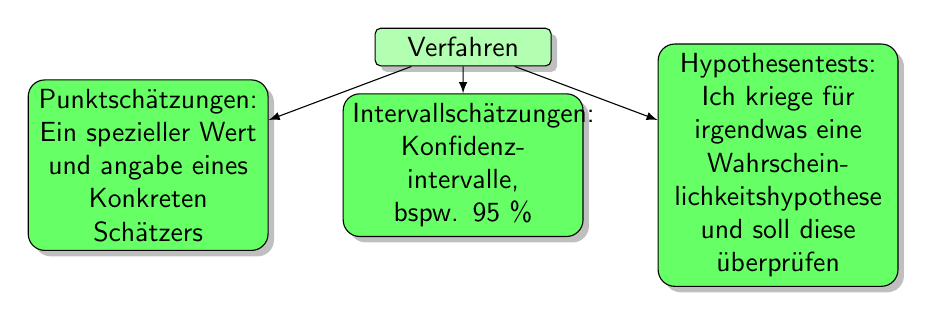
\begin{tikzpicture}[
level 1/.style={sibling distance=40mm},
edge from parent/.style={->,draw},
>=latex]

% root of the the initial tree, level 1
\node[root] {Verfahren}
% The first level, as children of the initial tree
child {node[level 2] (c1) {Punktschätzungen: Ein spezieller Wert und angabe eines Konkreten Schätzers}}
child {node[level 2] (c2) {Intervallschätzungen: Konfidenzintervalle, bspw. 95 \% }}
child {node[level 2] (c3) {Hypothesentests: Ich kriege für irgendwas eine Wahrscheinlichkeitshypothese und soll diese überprüfen}};

 
\end{tikzpicture}
\subsection{Maximum Likelihood Schätzung}
Was ist der beste Schätzer? Die Idee hier ist, dass man einen Schätzer derart wählt, dass dieser die gegebene Beobachtung mit der größtmöglichen Wahrscheinlichkeit erscheint. Die Formeln finden sich auf Seite 261
\subsection{Konfidenzintervall}
û untere Grenze ô obere Grenze.$\alpha$ ist der akzeptierte Fehler. Wir brauchen erstmal Punktschätzungen für die Parameter.\\
mögliche Settings:
\begin{enumerate}
	\item ich habe eine Varianz, dann gibt es das zweiseitige und das einseitige obere/untere Konfidenzintervall
	\item Varianz unbekannt: Ich ersetze die bekannte Varianz durch eine Schätzung (Stichprobenvarianz $\hat{\sigma}$)
	\item Konfidenzintervall für die Differenz zweier Erwartungswerte (bei unbekannter gleicher Varianz). Wenn Differenz negativ ist ein $\mu$ stets kleiner als das andere. Anwendung: Bspw. Fertigung und ich will wissen was besser ist.
\end{enumerate}
\subsection{Lineares Regressionsmodell}
Wir haben genauso wie in der Beschreibenden $x_1...x_n$ Werte mit unbekannter Varianz. $\varepsilon_i$ Sind Störterne, die $Y_j$ Werte sind genauso stoch. unabh. verteilt wie $\varepsilon$. Sigma kann ich mir auch herschätzen über 7.7. n-2 weil a und b geschätzt werden. \begin{landscape}
\section{Aufgabentypen}
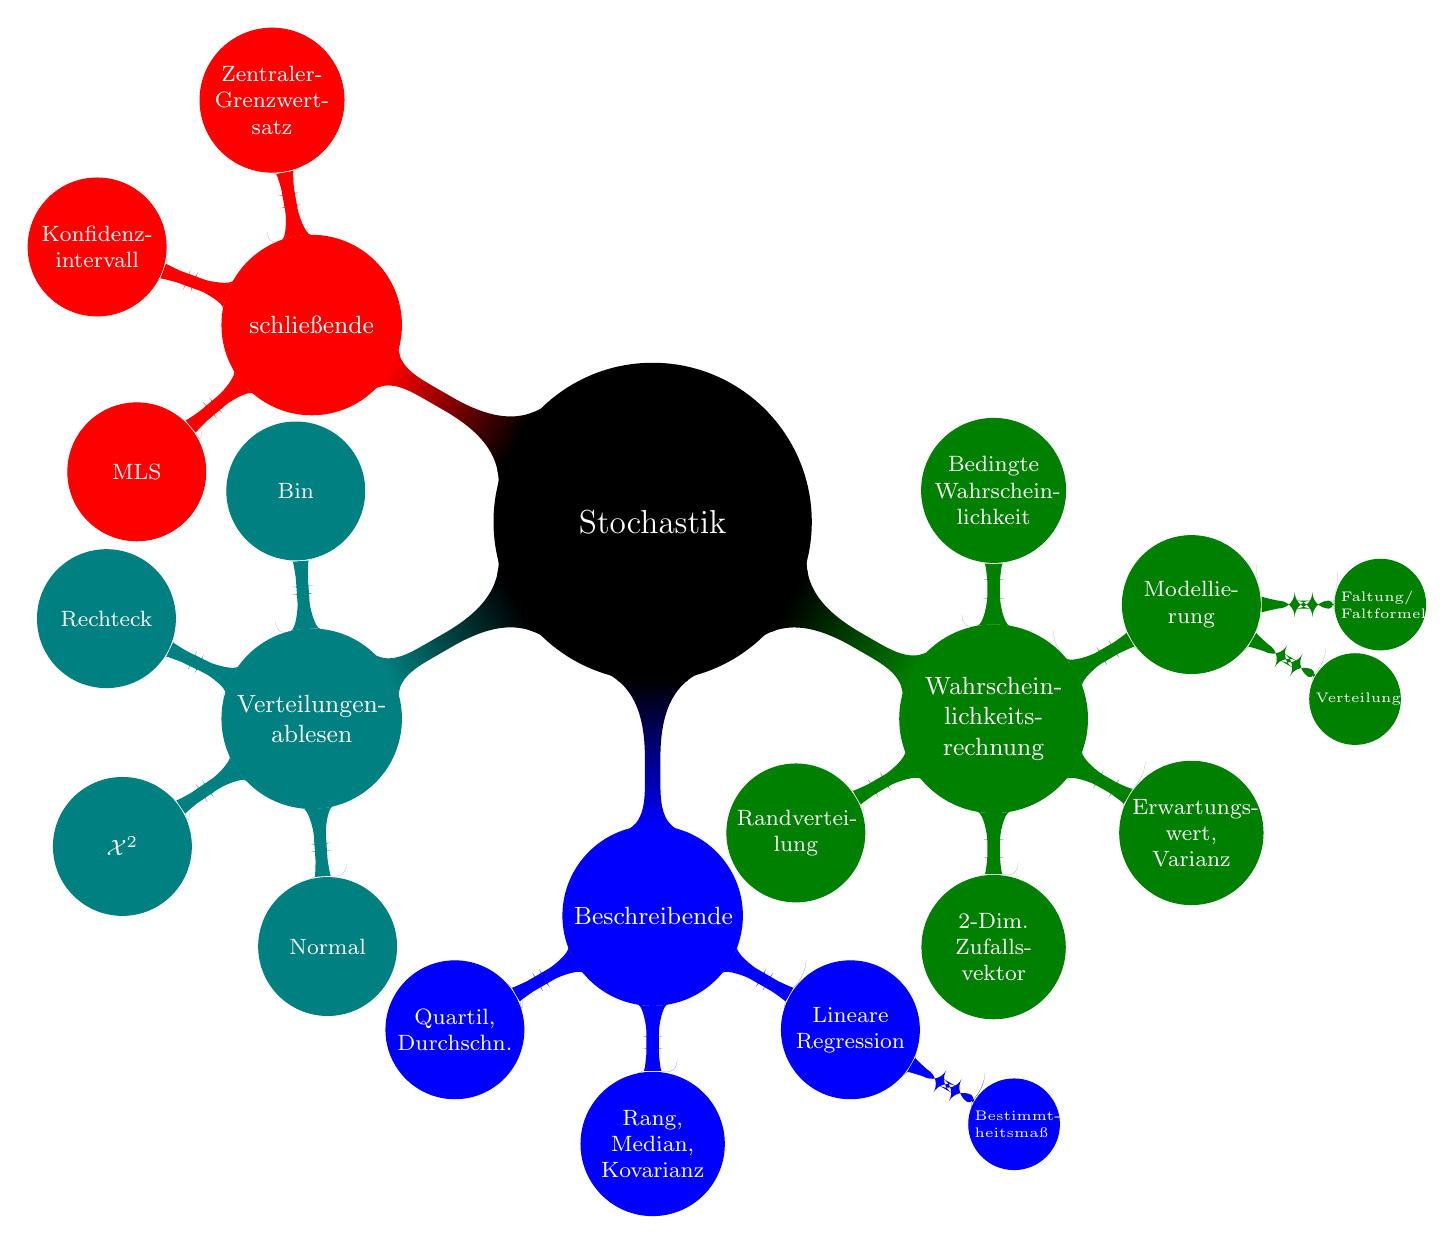
\begin{tikzpicture}
\path[mindmap,concept color=black,text=white]
node[concept] {Stochastik}
[clockwise from=-30]
child[concept color=green!50!black] {
	node[concept] {Wahrschein-\\lichkeits-\\rechnung}
	[clockwise from=90]
	child { node[concept] {Bedingte Wahrscheinlichkeit} }
	child { node[concept] {Modellie\-rung}[clockwise from=0]
		child[concept] {node[concept] {Faltung/ \\ Faltformel} }
	child {		node[concept] {Verteilung} }}
	child { node[concept] {Erwartungs\-wert, Varianz} }
	child { node[concept] {2-Dim.\\ Zufalls\-vektor} }
	child { node[concept] {Randvertei\-lung}}
}  
child[concept color=blue] {
	node[concept] {Beschreibende}
	[clockwise from=-30]
	child { node[concept] {Lineare Regression} 
			[clockwise from=-30]
		child[concept color=blue] {
			node[concept] {Bestimmt\-heitsmaß} }}
	child { node[concept] {Rang, Median,\\ Kovarianz} }
	child { node[concept] {Quartil,\\Durchschn.} }
}
	child[concept color=teal] { node[concept] {Verteilungen\-ablesen}  [clockwise from=274] 
		child { node[concept] {Normal} }
		child { node[concept] {$\mathcal{X}^2$} }
		child { node[concept] {Rechteck} }
		child { node[concept] {Bin} }
	}
child[concept color=red] { node[concept] {schließende} [clockwise from=220]
	child { node[concept] {MLS} }
	child { node[concept] {Konfidenz\-intervall} }
	child { node[concept] {Zentraler\-Grenzwert\-satz} }
	} 
	


;
\end{tikzpicture}
    \end{landscape}

\section{Globalübung last}
\subsection{Aufgabe 39}
Mit n=10 und $\alpha = 0.01$ erhält man aus der Quantiltabelle der $X^2$ Verteilung $X^2(n-1)=X^2_{0.01}(9) gerundet 2.09$\\
Weiter berechnet man aus dem gegebenen Daten $x_1\dots x_{10}$\\
$\bar{x} = \frac{1}{10} \sum_{i=1}^{10}xi =124.9$ und $\hat{\sigma^2}=\frac{1}{9}\sum_{i=1}^{10}$\\

b)\\ Es ergibt sich $K_{\sigma} = [0,\sqrt{\frac{n-1}{X^2_\alpha(n-1)}\hat\sigma^2}] \cong [0,4.837]$
\subsection{Aufgabe 40}
Lösung wird hochgeladen. $\sigma_{pool}$ ist sozusagen ein Schätzer für Sigma. \\Ansatz: Mit $n_1 = 12, n_2=8, 1-\alpha=0.95 \Leftrightarrow 1- \frac{k}{2} = 0.975$ erhält man aus der Quantil Tabelle der T-Verteilung $$t{1-\frac{\alpha}{2}} (n_1+n_2 - 2) = t_{0.975} (18) \approx 2.101 $$
Aus den Messwerrten $x_1\dots,x_{12}$ und  $y_1\dots,y_{8}$ berechnet man: 

$$\bar{x}=\frac{1}{12}\sum_{i=1}^{12} (x_i = 50.4) $$ $$\bar{y}\frac{1}{8}\sum_{i=1}^{8} y_i = 50.6$$ $$\hat{\sigma}=\bar {x}\bar{y}=-0.2$$

\subsection{Aufgabe 41}

Das erste was bei der Regressionsanalyse zu tun ist, ist das Erstellen einer Tabelle.\\
Mit Hilfe der Einträge in der letzten Zeile der Berechnungstabelle erhält man $$\bar{x} = \frac{1}{7}* 18.55=2.65$$ $$\bar{y}= \frac{1}{7}*42.7 = 6.1$$ 
$$S^2_x = \frac{1}{7}\sum_{i=1}^{7}x^2_i-\bar{x}^2 = 0.0136$$ 
$$S^2_y =\frac{1}{7}\sum_{i=1}^{7}y^2_i-\bar{y}^2\approx 0.1657$$
$$S_{xy} = \frac{1}{7}\sum_{i=1}^{7}x_i*y_i-\bar{x}\bar{y}\approx -0.0361$$\\
Hieraus ergeben sich gemäß A8.4 und D7.4 die folgenden kleinste Quadrate Schätzung:\\
$$\hat{b} = \frac{S_{xy}}{S^2_x} \approx -2.654$$
$$\hat{a} = \bar{y}-\hat{b}\bar{x}\approx13.133-2.654*2.65$$\\
Die ugehörige geschätzte Regressionsgerade ist somit 
$$\hat{y}(x)=\hat{a}+\hat{b}x\approx13.133-2.654x$$
Absatzmenge siehe Graphik (in 100 kg)\\~\\
Bei Zeichnungen in der Klausur drauf achten, dass die Achsen und Punkte richtig beschriftet sind.
\\~\\
c)
Mit $n=7$ und $1-\alpha = 0.9 \Leftrightarrow \alpha=0.1$ erhält man aus der Quantiltabelle der $X^2$Verteilung 
$$X^2_{\frac{x}{2}}(x-2)=X^2_{0.05}(5)\approx 1.15 $$ und 
$$X^2_{1-\frac{x}{2}}(n-2)=X^2_{0.95}(5)\approx11.09$$
Weiter folgt mit den Ergebnissen aus (a): 
$$\sigma^2 = \frac{n}{n-2}(S^2_y-\frac{S^2_{xy}}{S^2_x})=\frac{7}{5}(0.1657-\frac{(-0.0361)^2}{0.0136})\approx0.098$$
Man erhält das folgende zweiseitige 90\% Konfidenzintervall für $\sigma^2$ 
$$K_{\sigma^2}\approx[\frac{5*0.098}{11.07},\frac{5*0.098}{1.15}]\approx[0.044,0.426]$$
\section{Klausurinformationen aus letzter Vorlesung}
Die Aufgaben die man heute behandelt werden nicht den ganzen Stoff umfassen. Nicht darauf verlassen nur das zu können was präsentiert wird. Es gibt aber eine gewisse Sicherheit dass man besteht wenn man die Aufgaben kann.\\
Alle Aufgaben werden ins Netz gestellt, aber ohne Lösung.
\subsection{Aufgabe 1 Urlaub und Feriengäste}
\begin{enumerate}[label=(\alph*)]
	\item Welche Werte kommen überhaupt vor?\\
	\begin{tabular}{|c|c|c|c|c|c|}
		\hline a(1) & a(2) & a(3) & a(4) & a(5) & a(6) \\ 
		\hline 2 & 3 & 7 & 10 & 14 & 21 \\ 
		\hline 
	\end{tabular} \\~\\
	Zugehörige Tabelle der absoluten relativen und kummulierten relativen Häufigkeiten (abs Häufigkeiten mittels Auszählen der Urliste):\\
	\begin{tabular}{|c|c|c|c|}
		\hline Verweildauer & Absolute Häufigkeit & Relative Häufigkeit & Kumulierte relative Häufigkeit \\ 
		\hline 2 & 6 & 6/40=0.15 & 0.15 \\ 
		\hline 3 & 2 & 0.05 & 0.2 \\ 
		\hline 7 & 1 & 0.3 & 0.5 \\ 
		\hline 10 & 6 & 0.15 & 0.65 \\ 
		\hline 14 & 10 & 0.25 & 0.9 \\ 
		\hline 21 & 4 & 0.1 & 1 \\ 
		\hline 
	\end{tabular}\\
	Summe: 40=n\\~\\
	Gemäß Vorlesung ist nach (A2.5,A2.6)  die gesuchte empirische Verteilungsfunktion $F_{40}:\mathbb{R}\rightarrow[0,1]$ gegeben durch\\~\\
		$F_{40}=$
	$\begin{cases}
		0  & x < U(1)\\
		\sum_{j=1}^{k}f(j)  &  U(k) \leq x < U(k+1), k \in \{1,\dots, 5\}\\
		1 & x \geq u(6)\\
	\end{cases}$\\
	Die kumulierten relativen Häufigkeiten $$\sum_{j=1}^{k}f(j), k\in \{1,...,5\}$$ 
	Zu $ u(1),\dots,u(k+1)$ sind in der letzten Spalten der oben gezeigten Tabelle enthalten. Hiermit folgt: \\~\
	$F_{40}(x)= 
	\begin{cases}
		0 & x<2\\
		0.15 & 2\leq x <3\\
		0.2 & 3\leq x < 7\\
		0.5 & 7 \leq x <10\\
		0.65 & 10 \leq x <14\\
		0.9 & 14 \leq x < 21\\
		1 & 21 \leq x\\
	\end{cases}$\\
	Das kann man auch umgekehrt machen, es kann sein dass man so eine Grafik gegeben hat mit den Stufen und daraus rekonstruiren. Ich kann die relativen Häufigkeiten ablesen aus den Sprunghöhen. 100\% KLAUSUR!
	\item Berechnung der gesuchten Anteile mittels der empirischen Verteilungsfunktion. \\~\\Anteil der Gäste mit höchstens 14 Tagen Verweildauer $F_{40}(14)=0.9$ (einfach ablesen, geht aus aus der Graphik).\\~\\
	Anteil der Gäste mit mehr als 7 Tagen Verweildauer = $1-F_{40}(7)= 1-0.5=0.5$\\~\\
	Anteil der Gäste mit mindestens 3 Tagen, aber höchstens 14 Tagen Verweildauer: $$F_{40}(14)-F_{40}(3)-\lim f_{40}(3)$$ d.h. Anteil der Beobachtungen im Intervall[3,14] + Anteil der Beobachtungen die =3 sind
	$$= F_{40}(14)-F_{40}(2) = 0.9-0.15 = 0.75 $$
	

\end{enumerate}
\subsection{Aufgabe 2}
\begin{enumerate}[label=(\alph*)]
	\item Zuerst der einfache Fall: 
	Für $x\in [-\infty,0]$ gilt 
	$$f^X(x)= \int_{-\infty}^{\infty}f^{(x,y)}(x,y)dy=0$$
	Für $x\in (0,\infty)$ gilt
	$$f^X(x)= \int_{- \infty}^{\infty} f^{(x,y)} (x,y)dy $$
	
	$$\overset{\text{nach Voraussetzung}}{=} \int_{x}^{x+2}\frac{1}{2} e^{-x} dy = \frac{1}{2} e^{-x} (x+2-x) = \frac{1}{2} e^{-x} *2 = e^{-x}$$\\
	Insgesamt:\\
	(1) $ f^X(x)=\begin{cases}
	e^{-x} & x\in (0,\infty)\\
	0 & \text{sonst}\\
	\end{cases} $\\~\\somit gilt $X \sim Exp(1)$
	
	\item Gemäß B 3.4 gilt: (Tipp hinschreiben für was die Grenzen sind an den eckigen Klammern)
	$$P(1<X\leq 2) = \int_{1}^{2}f^X(x)dx \overset{\text{nach 1}}{=} \int_{1}^{2}e^{-x}dx$$
	$$\left[-e^{-x}\right]^{x=2}_{x=1} = -e^{-2}+e^{-1}=e^{-1}-e^{-2} $$
	
	\underline{Alternativlösung zu b:}\\
		Gemäß (a) und B3.7 gilt für die Verteilfunktion $F^x$ von X:\\ $ F^X (x) \begin{cases} = 0 & \text{ für } x \in [-\infty,0]\\ 1-e^{-x} &  x \in (0,\infty)\\ \end{cases}$\\~\\
	Hiermit folgt $P(1<X \leq 2) \overset{C 2.4}{=}  F^X(2)- F^X(1)= 1-e^{-2} - (1-e^{-1}) = e^{-1} - e^{-2}$\\
	
	
	\item Sei $x\in (0,\infty).$ Dann gilt gemäß (1) 
	
	$$f^X(x)=e^{-x}>0$$ Es folgt für $y\in [x,x+2]$\\
	(2) $ f^{Y|X=x}(y) \overset{\text{nach C7.1}}{=} (4) \frac{f^{X,Y}(x,y)}{f^X(x)} \overset{\text{nach Vor. (1)}}{=}  \frac{1/2 e^-x}{e^-x} = 1/2$\\~\\
	
Für $y \in \mathbb{R} \backslash  (x, x+2) = 2$ folgt\\
(3) $f^{Y|X=x}(y) = nach 7.1 f^(x,y)/f^x(x) = 0$

Insgesamt folgt aus (2),(3)\\

(4)$f^{Y|X}=x(y) =  \begin{cases}
	\frac{1}{2} &  y \in <[x,x+2]\\
	0 & sonst\\
\end{cases}$\\

Gemäß B 3.6 ist dies die Dichte der Rechteck-Verteilung R[x,x+2]

\item Für $x\in (0,\infty)$ gilt:\\
$$E(Y|X=x) \overset{\text{nach C. 7.4}}{=}  \int_{-\infty}^{\infty} y f^{Y|X=x}(y)dy$$

$$\overset{\text{nach (4)}}{=}  \frac{1}{2}  \int_{x}^{x+2}y dy = 1/2\;\left[y^x /2\right]^{x+2}_x $$\\

$1/4((x+2)^2-x^2 - x^2) =  1/4$\\~\\
\underline{Alternativlösung zu d):}\\~\\
 	Gemäß (c) gilt $P^{Y|X=x} = R[x,x+2]$ für $x>0$. Hierraus folgt mit C 5.2, (iii). $$E(Y|X=x) = \frac{x+(x+2)}{2} = \frac{2x+2}{2}=x+1$$
	
	\item in der Klausur kann sein dass eine Randdichte und eine bedingte Dichte gegeben ist und wir daraus die gemeinsame Dichte berechnen müssen (sollte aber nicht so schwer sein.)
\end{enumerate}


Sonderinfo: X, Y stoch unabhängig E(XY) =  E(X)E(Y), Kovarianz =0, da E(XY)-E(X)E(Y)

Klausur: Es kann sein dass irgendwo eine Modelierung drankommt, wo ich eine reale Situation abbilden muss (wie in der nächsten Aufgabe).
\subsection{Aufgabe 3}
\begin{enumerate}[label=(\alph*)]
	\item Modellierung: Die Anzahlen der Münzen in $n\in \mathbb{N}$ Rollen können beschrieben werden durch stochastisch unabhängige identisch verteilte Zufallsvariabeln $X_1\dots X_n$\\~\\
	Zugehörige Interpretation für $i \in \{1,\dots , n\}$\\
$X_i$ gibt die Anzahl der Münzen in Rolle an. Gemäß Voraussetzung ist die Wahrscheinlichkeitsverteilung von $X_i$ für $i \in \{1,\dots ,  n \}$ gegeben durch folgende Tabelle (1)\\~\\
\begin{tabular}{|c|c|c|c|c|}
	\hline $k$ & 48 & 49 & 50 & 51 \\ 
	\hline $P(X_i=k)$ & 0.1 & 0.2 & 0.6 & 0.1 \\ 
	\hline 
\end{tabular} \\~\\
Hierbei Interpretation der gegebenen Prozentanteile als gesuchte Wahrscheinlichkeiten. Aus der angegebenen Verteilung folgt für $i \in \{1,\dots,n\}$:\\~\\
$$(2)\; \mu = E(X_i) = \sum_{k=48}^{51}k*P(X_i=k) \overset{(nach 1)}{=}  48*0.1*49*0.2+50*0.6+51*0.1=49.7$$\\~\\
$$(3)\; \sigma^2 = Var(X_i) = E(X_i^2 - (E(X_i)^2)) = \sum_{k=48}^{51}k^2 P(X_i=k)- \mu^2 =48^2*0.1+49^2*0.2+50^2.... = 0.61$$

\item Gesucht: $P(49 670 \leq S_n \leq 49 730)$ mit $n=1000$ und $S_n = \sum_{i=1}^{n}X_i$, d.h. Gesamtwert in $n=1000$ Rollen\\~\\
Es gilt $P(49 670\leq S_n \leq 49 730) = P(S_n  \leq 49 730) - P(S_n < 49 670) =  P(S_n \leq 49669)$\\
$$= P(\frac{S_n-u\mu}{\sqrt{n*\sigma^2}}\leq \frac{49730-u\mu}{\sqrt{n*\sigma^2}}) - P(\frac{S_n-u\mu}{\sqrt{n*\sigma^2}}\leq \frac{49669-u\mu}{\sqrt{n*\sigma^2}})$$ 
$$\approx \Phi (\frac{49730-n\mu}{\sqrt{n*\sigma^2}}- \Phi (\frac{49669-n\mu}{\sqrt{n*\sigma^2}})$$\\
$$=\Phi(1.21)-(1-\Phi(1.26)) $$

$$\approx 0.887 + 0.896 - 1 = 0.783$$
\end{enumerate}
\subsection{Aufgabe 4 Maximum Likelihood Schätzung}
Seien $x_1,\dots,x_n > 0 $ Realisationen von $X_1,\dots,X_n$\\
Die zugehörige Likelihood Funktion gemäß Definition 3.2\\
$$(1) L(\alpha|x_1,\dots,x_n) \overset{\text{unabh.}}{=} \prod_{i=1}^{n}f_d(x_i)$$ \\ 
$$\overset{\text{nach definiton von }f \alpha}{=}  \prod_{i=1}^{n} \frac{1}{\alpha} e^{-\frac{x_i}{d}}$$
$$= (\frac{1}{\alpha})^n exp(- \frac{1}{\alpha} \sum_{i=1}^{n} x_i)$$ \\~\\
Zugehörige Log-Likelihood Funkion (Kommentar: mit dieser ist einfacher zu rechnen)\\
$$l(\alpha) = ln (L(\alpha|x_1,\dots,x_n))$$ 
$$= ln((\frac{1}{\alpha})^n) - \frac{1}{\alpha} \sum_{i=1}^{n} x_i $$
$$=-n*ln(\alpha) - \frac{1}{\alpha}\sum_{i=1}^{n}x_i,\alpha \in (0,\infty) $$ 
Gemäß (2) ist l diferenzierbar auf $\int(0,\infty)$ mit\\ (3) $$l'(\alpha) = - \frac{n}{\alpha} - \sum_{i=1}^{n} x_i (\frac{-1}{\alpha^2})$$
$$\frac{-n}{\alpha} + \frac{1}{\alpha^2}\sum_{i=1}^{n}x_i $$
$$= \frac{-n}{\alpha} + \frac{1}{\alpha^2} n \bar{x} = \frac{n}{\alpha^2}(\bar{x}\alpha) $$
$$\begin{cases}
>0 & \text{ , falls } \alpha < \bar{x}\\
= 0 & \text{ , falls } \alpha = \bar{x}\\
<0 & \text{ , falls } \alpha > \bar{x}\\
\end{cases}$$
\\~\\
Aus (3) folgt, dass l streng monoton wachsend auf $(0,\bar{x}]$ und streng monoton fallend auf $[\bar{x},\alpha)$ ist. Somit besitzt die Log-Likelihood Funktion $\alpha \rightarrow L(\alpha| x_1,\dots , x_n)$ selbst ein eindeutig bestimmtes \underline{globales} Maximum in $\hat{\alpha} = \bar{x}$\\~\\
D.h. Maximum Likelihood Schätzung zu $\alpha$ gegeben durch $$\hat{\alpha} = \bar{x}$$


Klausurtipp:  Nicht die zweite Ableitung ausrechnen und dann untersuchen, dauert zu lange.

\subsection{Aufgabe 5}
Gemäß D 5.9 ist ein einseitiges unteres konfidenzintervall für die Varianz $\sigma^2$ (bei unbekanntem $\mu$) zum Konfidenzniveau 1-$\alpha \in (0,1)$ gegeben durch 
$$\mathcal{K}= \left[0,\frac{n-1}{\mathcal{X}^2_{\alpha}(n-1)} \hat{\sigma}^2 \right]$$
$$\hat{\sigma}^2 = \frac{1}{n-1} \sum_{i=1}^{n} (x_i - \bar{x})^2 \text{ ist hierbei die Stichprobenvarianz zu } x_1\dots,x_n$$
\underline{Einsetzen der Zahlenwerte}:\\
Mit $n=10$ und $1-\alpha = 0.9 \Leftrightarrow \alpha = 0.1$ Erhält man aus der Quartilstabelle der $\mathcal{X}^2$ - Verteilung.\\~\\
Mit n=10 und $1-\alpha = 0.9 \Leftrightarrow \alpha = 0.1$ erhält man aus der Quantil-Tabelle der $\mathcal{X}^2$-Verteilung:
$$\mathcal{X}^2_{\alpha}(n-1) = \mathcal{X}^2_{0.1}(9) \overset{Tabelle}{\approx} 4.17$$
Weiter berechnet man aus $x_1\dots, x_{10}$
$$\bar{x} = \frac{1}{10} \sum_{i=10}^{10} x_i = 149$$ und
$$\hat{\sigma}^2 = \frac{1}{9} (\sum_{i=1}^{10} x^2_i - 10 \bar{x}^2) = 10$$
Hiermit folgt: 
$$\mathcal{K}= [0,\frac{9*10}{4.17}] \approx [0,21.583]$$
Das ist der Fall 1 wo Stichprobe und normalverteilte Daten und gesucht ist.. Eine andere Situtation (Klausur!!!) ist Regressionsmodell und Freiheitsgrad ist n-2, da ist es eine andere Rechnung.

\subsection{Letzte Tipps}
\begin{itemize}
	\item Bezeichnungen kennen, z.B.: $P(X=2,Y=5)$ ist unterschiedlich gegenüber $P(X=2|Y=5)$
	\item Was bedeutet $f^{X,Y}(x,y)$ gegenüber $f^{Y|X=x}(y)$
	\item Standardaufgaben:
	\begin{itemize}
		\item Bestimmung von Maximum Likelihood Schätzungen
		\item Anwendung des Zentralen Grenzwertsatzes
		\item Berechnungen zu 2-Dimensionalen Zufallsvektor(X,Y) (diskret und stetig)
		\item Anwendung der Rechenregeln zu Erwartungswert, Varianz, Kovarianz
		\item Faltung von Zufallsvariabeln
	\end{itemize}
	\item Standardaufgaben zur deskriptiven Statistik (vgl Übungen)
	\item Stochastische Unabhängigkeit und deren Anwendungen z.B. $E(XY) = ?$
	\item Integration (einfacher) Funktionen (auch Doppelintegrale)
	$$\int_{0}^{\infty} x*2e^{-2x} dx \overset{\text{nach Buch}}{=} \frac{1}{2} $$
	Dichte zu Exp(2) an der Stelle $x = E(Z)$ mit $Z \sim Exp(2)$
	\end{itemize} 
\end{document}